\section{Combined Energy Scale}
\label{secCES}

Scintillation and ionization signals produced in liquid xenon by ionizing radiation can be simultaneously observed with high efficiencies. A strong anti-correlation between them can be measured and used to improve the energy resolution, since the fluctuation of their sum is smaller than that of individual signals.

%The strong anti-correlation between charge and light has been observed in liquid argon. 
The `macroscopic' anti-correlation between scintillation and ionization in a double phase xenon detector can be observed by varying the electric field~\cite{CES_Kubota}. The proportion of light and charge is different at different drift fields, but their sum is constant~\cite{CES_Conti, CES_Aprile}, as shown in Fig.~\ref{figMicroMacro_1}. Only at very low electric fields some deviation can be observed due to electron attachment to electronegative gases and a moderate recombination rate. In analogy to the macroscopic anti-correlation, the energy shared  between scintillation and ionization also fluctuates on an event basis, which results in `microscopic' anti-correlation shown in Fig.~\ref{figMicroMacro_2}. Both effects are related to the fixed number of electron-ion pairs and excitons produced per unit of energy deposition.

\begin{figure}[!h]
\centering
\subfigure[`macroscopic' anti-correlation]{
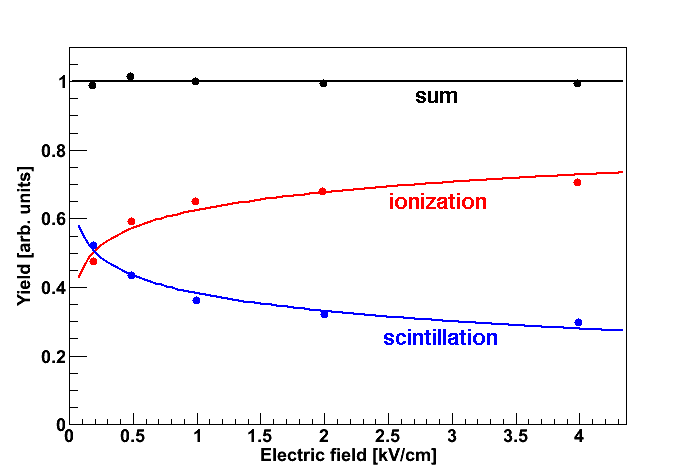
\includegraphics[width=0.475\linewidth]{plots/CES/MacroscopicAnticorrelation_withLabels.png}
\label{figMicroMacro_1}}
\subfigure[`microscopic' anti-correlation]{
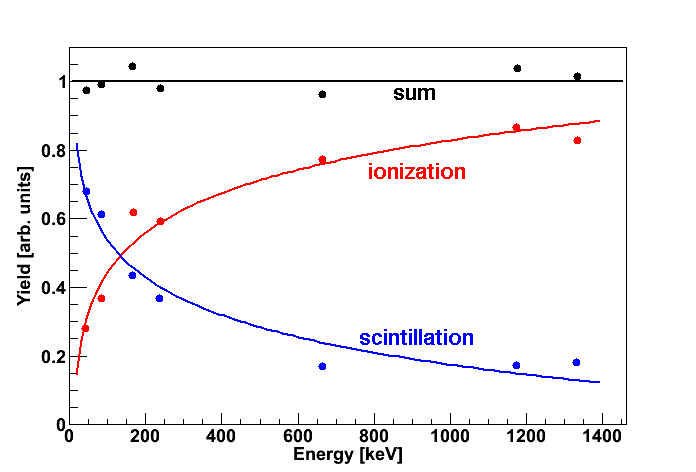
\includegraphics[width=0.475\linewidth]{plots/CES/MicroscopicAnticorrelation_withLabels.png}
\label{figMicroMacro_2}}
\caption[Macroscopic and microscopic anti-correlation between scintillation light and ionization]{(a) - macroscopic anti-correlation between scintillation light and ionization as a function of electric field. Data points from Ref.~\cite{CES_Conti}. (b) - microscopic anti-correlation between light and charge as a function of the $\gamma$-photon energy at drift field of 0.53~kV/cm. Data  points from Ref.~\cite{TeresaInternal}. }
\label{figMicroMacro}
\end{figure}

Due to the anti-correlation between charge and light, the energy resolution of a double-phase xenon detector can be significantly improved by combining the signals from scintillation and ionization channels into a new energy scale, which is independent from the drift field and particle energy.

The distribution of S1 and S2 signals for $^{137}$Cs data taken with an anode voltage of 4.5~kV (standard operation voltage of XENON100) is shown in a two-dimensional plot in Fig.~\ref{figCES_S2vsS1_Cs137}. Only the bottom S2 signal has been considered in order to avoid problems related to PMT saturation (see Section~\ref{secPosRecSaturation}), and the S2 scale is approximately normalized to S1, by applying a scaling factor 5$\times$10$^{-3}$. 
The population corresponding to the 662~keV peak can be fitted with a two-dimensional elliptical Gaussian function:

\begin{equation}
f(x,y) = A \cdot e^{-(a(x-x_{0})^{2} + 2b(x-x_{0})(y-y_{0}) + c(y-y_{0})^{2})},
\end{equation}
where $A$ - peak height, and the equation in the brackets is an implicit equation of an ellipse with $x_{0}$ and $y_{0}$ - the coordinates of the center of the distribution (mean of S1 and S2 signals in [PE]),

\begin{equation}
\nonumber
a = \frac{\cos^2{\Theta}}{2\sigma^{2}_{x}} + \frac{\sin^2{\Theta}}{2\sigma^{2}_{y}}, \ \
b = \frac{\sin{2\Theta}}{4\sigma^{2}_{x}}-\frac{\sin{2\Theta}}{4\sigma^{2}_{y}}, \ \
c = \frac{\sin^2{\Theta}}{2\sigma^{2}_{x}}+\frac{\cos^2{\Theta}}{2\sigma^{2}_{y}},
\end{equation}
and 
$\sigma_{x}$ and $\sigma_{y}$ - standard deviation of S1 and S2 signals [PE], respectively; $\Theta$ - rotation angle.


%\begin{floatingfigure}[l]{0.4\textwidth}
\begin{figure}[!h]
\centering
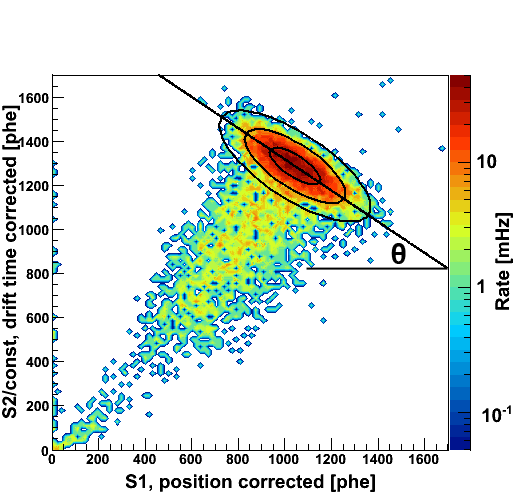
\includegraphics[height=0.4\linewidth]{plots/CES/662keV_const200_withFits_withLabels.png}
\caption[Anti-correlation between prompt (S1) and proportional (S2) scintillation signals for $\gamma$-rays from a $^{137}$Cs source]{Anti-correlation between prompt (S1) and proportional (S2) scintillation signals for $\gamma$-rays from a $^{137}$Cs source. Only the bottom S2 signal has been used in order to avoid problems related to PMT saturation (see Section~\ref{secPosRecSaturation}). The ellipses show 1$\sigma$, 2$\sigma$ and 3$\sigma$ contours of the elliptical gaussian fit. The black lines show the  anti-correlation angle $\Theta$.}
\label{figCES_S2vsS1_Cs137}
\end{figure}
%\end{floatingfigure}


% defined with a following equation with 6 free parameters (height of the peak, mean X, mean Y, sigma X, sigma Y and rotation angle Theta)
The combined energy scale (CES) is obtained by projecting the two-dimensional distribution along the major axis of the anti-correlation ellipse~\cite{CES_Aprile}:

\begin{equation}
\label{eqCES}
\mathrm{CES} = \frac{\mathrm{S1} \cdot \sin^2{\Theta} + \mathrm{S2} \cdot \cos^2{\Theta}}{\nu \cdot (\sin{\Theta} + \cos{\Theta})},
\end{equation}
where $\nu$ - coefficient used to normalize the new scale to the energy in [keV]. This CES is typically presented in a shorter definition
\begin{equation}
\label{eqCES1}
\mathrm{CES} = \mathrm{S1} \cdot \alpha + \mathrm{S2} \cdot \beta,
\end{equation}
where $\alpha$ and $\beta$ - scaling factors for S1 and S2, which take into account both anti-correlation angle and the energy normalization constant.

\begin{figure}[!h]
\centering
\subfigure[40 and 80 keV]{
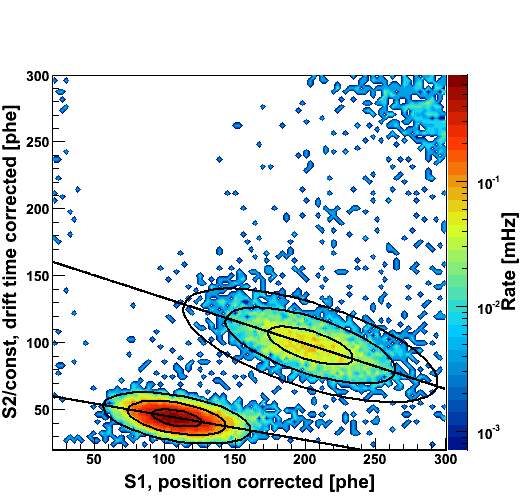
\includegraphics[height=0.4\linewidth]{plots/CES/40and80keV_const200_withFits.png}
\label{figCES_S2vsS1_1}}
\subfigure[164 and 236 keV]{
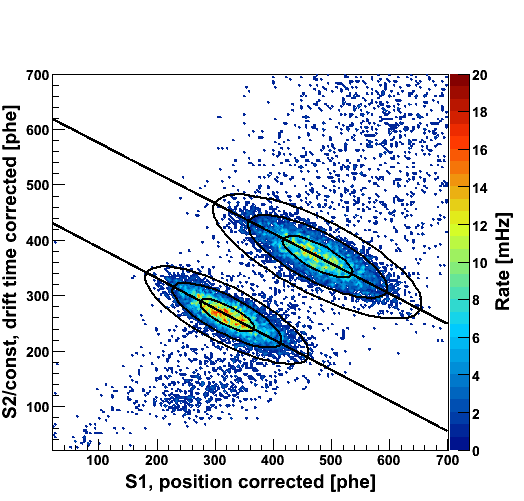
\includegraphics[height=0.4\linewidth]{plots/CES/164and236keV_const200_withFits.png}
\label{figCES_S2vsS1_2}}
%\subfigure[]{
%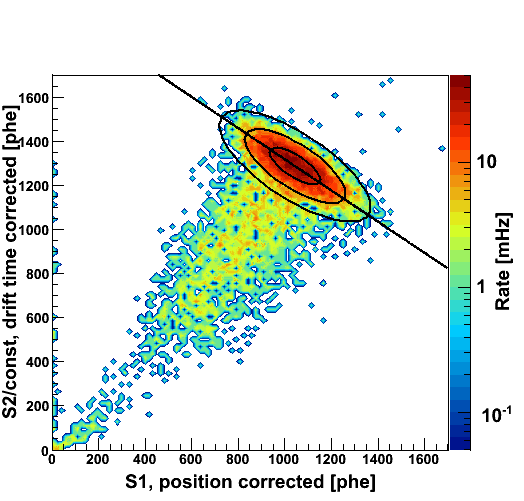
\includegraphics[width=0.3\linewidth]{plots/CES/662keV_const200_withFits.png}
%\label{figCES_S2vsS1_3}}
\caption[Anti-correlation between prompt and proportional scintillation signals for gammas of different energy]{Anti-correlation between prompt (S1) and proportional (S2) scintillation signals for gammas of different energy: (a) - 40~keV and 80~keV lines from inelastic neutron scattering on $^{129}$Xe and $^{131}$Xe, respectively. (b) - 164~keV and 236~keV from de-excitation of $^{131\mathrm{m}}$Xe and $^{129\mathrm{m}}$Xe.}
\label{figCES_S2vsS1}
\end{figure}

The analysis has been also performed for the lines with energies of 40~keV and 80~keV, from the inelastic neutron scattering on $^{129}$Xe and $^{131}$Xe, and for the 164~keV and 236~keV lines from the de-excitation of neutron-activated $^{131\mathrm{m}}$Xe and $^{129\mathrm{m}}$Xe. The S1 and S2 distributions are shown together with the two-dimensional Gaussian fits in Fig.~\ref{figCES_S2vsS1}. The results of the fits for all lines are presented in Table~\ref{tabCESresults}.

\begin{table}[!h]
\centering
\caption[Results of elliptical Gaussian fits describing the S2 vs S1 distribution for $\gamma$-rays with different energies]{Results of elliptical fits Gaussian describing the S2 vs S1 distribution for $\gamma$-rays with different energies. The anti-correlation angle $\Theta$ is calculated for S2 normalized to S1 using a scaling factor of 5$\times$10$^{-3}$.}
\label{tabCESresults}
%\vspace{0.2cm}
\begin{tabular}{>{\footnotesize}r |>{\footnotesize} r |>{\footnotesize} r |>{\footnotesize} c |>{\footnotesize} c |>{\footnotesize} c}
%\begin{tabular}{r | r | r | c | c | c}
\hline
de-excitation energy 	& S1	[PE]		& S2	[PE]					& S1 yield [PE/keV]		& S2 yield [PE/keV]		& $\Theta$ [$^{\circ}$] \\
%[keV] 			& [phe]		& [phe]					& [phe/keV]			& [phe/keV]			& [$^{\circ}$] \\
\hline
40~keV			& 108.4 		& 8.8	$\times$10$^{3}$		& 2.71				& 218.6 				& 10.5$\pm$0.2 \\
80~keV			& 202.8 		& 19.7$\times$10$^{3}$		& 2.54				& 246.1 				& 17.6$\pm$1.1 \\
164~keV			& 320.5 		& 52.9$\times$10$^{3}$		& 1.95				& 322.7 				& 28.9$\pm$0.5 \\
236~keV			& 475.9 		& 74.1$\times$10$^{3}$		& 2.02				& 314.0 				& 28.6$\pm$0.7 \\
662~keV			& 1043.3 		& 257.3$\times$10$^{3}$		& 1.58				& 388.6 				& 38.8$\pm$0.5 \\
\hline
\end{tabular}
\end{table}

The combined energy scale has been defined for $^{137}$Cs calibration data as:

\begin{equation}
\label{eqCES_Cs}
\mathrm{CES_{Cs}\ [keV]} = \mathrm{S1}_{\mathrm{total}} \cdot 0.266 + \mathrm{S2}_{\mathrm{bottom}} \cdot (1.795\times10^{-3}).
\end{equation}
The $^{137}$Cs energy spectrum reconstructed using this scale is shown together with the Monte Carlo simulation in Fig.~\ref{figCES_Cs137}, for the entire target volume with and without veto coincidence cut. The simulated spectrum has been convoluted with the measured energy resolution, described in Section~\ref{secEnergyResolution}. The measurement and simulation are in a very good agreement when the veto cut is not applied, including the low energy region with the xenon K-shell X-ray at $\sim$30~keV. With the veto coincidence cut, a slight discrepancy has been observed for the Compton part of the spectrum, resulting from uncertainties of the veto efficiency measurements( see Section~\ref{secVetoEfficiencyMeasurement}).

\begin{figure}[!h]
\centering
\subfigure[without veto cut]{
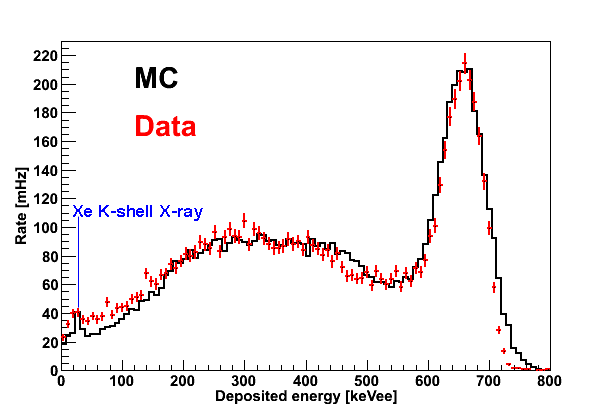
\includegraphics[height=0.3\linewidth]{plots/CES/Cs137_PassiveVeto_withXray.png}
\label{figCES_Cs137_1}}
\subfigure[with veto concidence cut]{
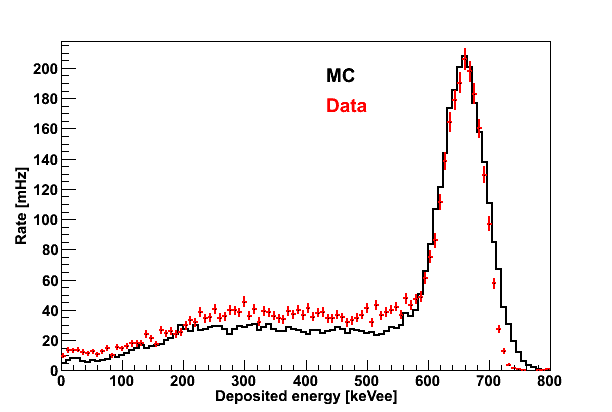
\includegraphics[height=0.3\linewidth]{plots/CES/Cs137_ActiveVeto.png}
\label{figCES_Cs137_2}}
\caption[Simulated and measured energy spectra for $^{137}$Cs in the entire target volume, without and with veto coincidence cut]{Simulated and measured energy spectra for $^{137}$Cs in the entire target volume, without (a) and with (b) veto coincidence cut. The measured spectrum has been reconstructed using combined energy scale. The xenon K-shell X-ray can be seen at the edge of the target volume. A slight discrepancy between Monte Carlo and measurement with the veto coincidence cut is due to uncertainties of the veto efficiency measurements (see Section~\ref{secVetoEfficiencyMeasurement}).}
\label{figCES_Cs137}
\end{figure}

\begin{figure}[!h]
\centering
\subfigure[]{
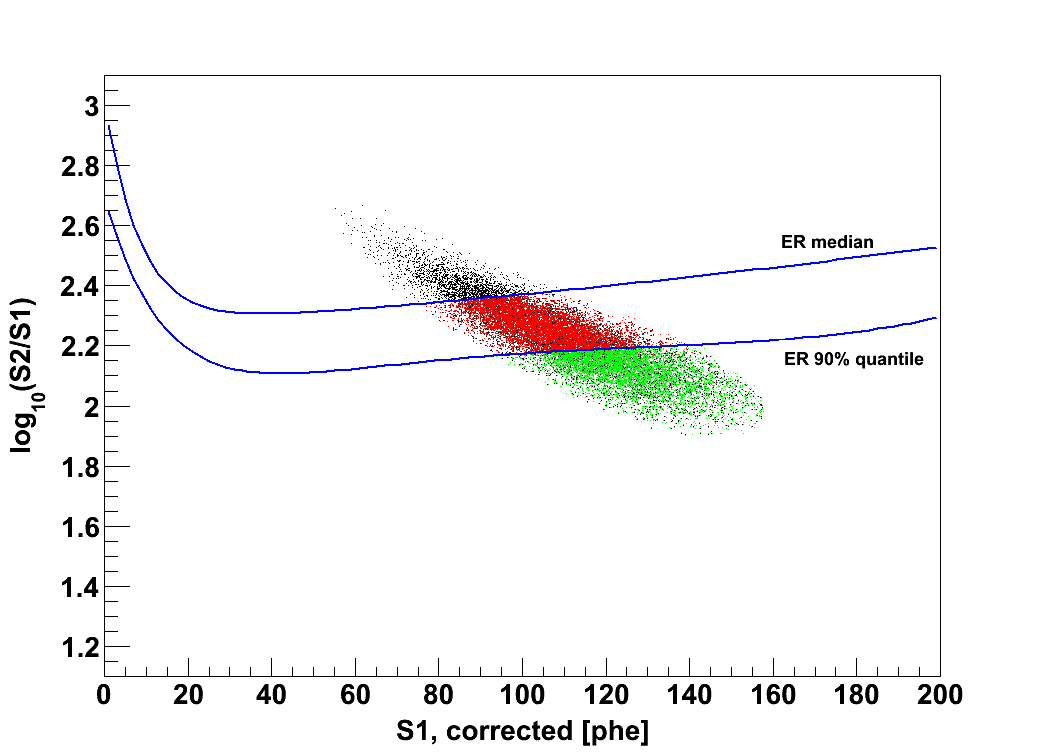
\includegraphics[height=0.3\linewidth]{plots/CES/logS2S1_40keV.png}
\label{figCES_AmBe_1}}
\subfigure[]{
%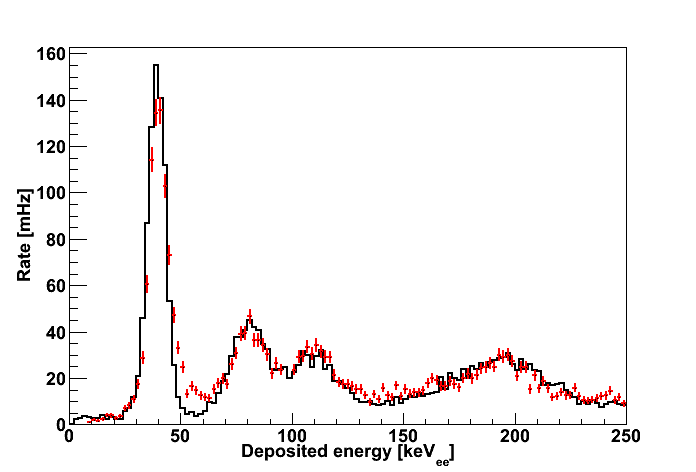
\includegraphics[height=0.3\linewidth]{plots/AmBeCalibration/AmBe_run0708_dataMC_0-250keV.png}
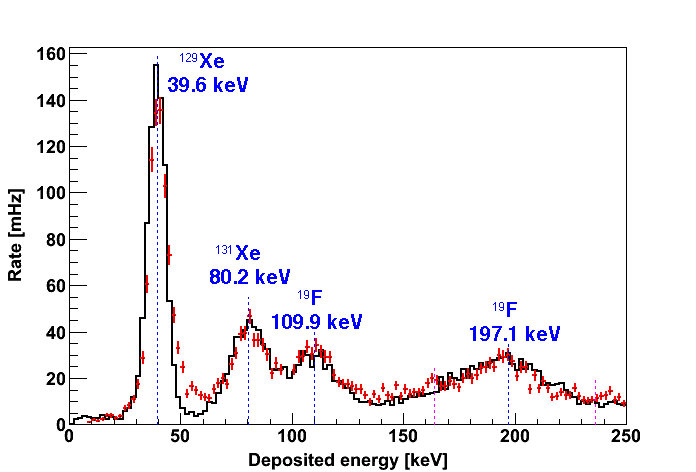
\includegraphics[height=0.3\linewidth]{plots/AmBeCalibration/CES_AmBe_withLinesAndLabels.png}
\label{figCES_AmBe_2}}
%\caption[The position of the 40~keV line from inelastic neutron scattering on $^{129}$Xe in respect to the electronic recoil band, and simulated and measured spectra for $^{241}$Am-Be calibration data in the entire target volume]{(a) - the position of the 40~keV line from inelastic neutron scattering on $^{129}$Xe in respect to the electronic recoil band. Due to contribution from nuclear recoils, the fraction of events below the ER median is 88.8\%, and 37.8\% of events are below the 90\% quantile. (b) - simulated and measured spectra for $^{241}$Am-Be calibration data in the entire target volume. Due to the contribution of nuclear recoils, a different definition of combined scale has been used to reconstruct the 40~keV and 80~keV peaks. The 110~keV and 197~keV originate from inelastic neutrons scatters in the PTFE of the TPC walls and can be observed only at the very edge of the target volume. The 164~keV and 236~keV $\gamma$-lines from de-excitation of $^{131m}$Xe and $^{129m}$Xe cannot be seen due to the short time of the dataset (1.09~days) and relatively long live times of the isotopes (8.88~days and 11.84~days, respectively).}
\caption[The position of the 40~keV line from inelastic neutron scattering on $^{129}$Xe in respect to the electronic recoil band, and the simulated and measured spectra for $^{241}$Am-Be calibration data in the entire target volume]{(a) - the position of the 40~keV line from inelastic neutron scattering on $^{129}$Xe with respect to the electronic recoil band (see Section~\ref{secBandCalibration}). Due to contribution from nuclear recoils, the fraction of events below the ER median is 88.8\%, and 37.8\% of events are below the 90\% quantile. (b) - simulated and measured spectra for $^{241}$Am-Be calibration data in the entire target volume. Due to the contribution of nuclear recoils, a different definition of combined scale has been used to reconstruct the 40~keV and 80~keV peaks. The 110~keV and 197~keV originate from inelastic neutrons scatters in the PTFE of the TPC walls and can be observed only at the very edge of the target volume. The 164~keV and 236~keV lines from de-excitation of $^{131\mathrm{m}}$Xe and $^{129\mathrm{m}}$Xe cannot be seen due to the short measuring time of the dataset (1.09~days) and relatively long live times of the isotopes (8.88~days and 11.84~days, respectively).}
\label{figCES_AmBe}
\end{figure}

As can be seen from Fig.~\ref{figCES_S2vsS1} and Table~\ref{tabCESresults}, the anti-correlation angle changes with energy. Thus, the definition of the combined energy scale computed on $^{137}$Cs data does not provide the proper reconstruction of the low energy lines in $^{241}$Am-Be data, and gives a worse energy  resolution. For 40~keV and 80~keV lines, this is caused to the contribution of the nuclear recoils, detected simultaneously with the electronic recoil from the de-excitation. They produce more ionization and less scintillation signal than `pure' electronic recoils, and the events are distributed mostly below the electronic recoil band (see Section~\ref{secBandCalibration}), with 88.8\% below the mean, and 37.8\% below the 90\% quantile, as shown in Fig.~\ref{figCES_AmBe_1}. The 110~keV and 197~keV peaks from inelastic neutron scatters on $^{19}$F in the PTFE walls of the TPC can be seen only at the very edge of the target volume, where the LCE for the S2 signal decreases abruptly (Section~\ref{secLCEs2}), and the quality of the spatial corrections might be worse. Thus, for the spectrum shown in Fig.~\ref{figCES_AmBe_2}, two different definitions of the combined scale have been used:
\begin{equation}
\label{eqCES_AmBe1}
\mathrm{CES_{AmBe_{1}}\ [keV]} = \mathrm{S1}_{\mathrm{total}} \cdot 0.250 + \mathrm{S2}_{\mathrm{bottom}} \cdot (5.807\times10^{-3}), \text{ below $\sim$100~keV},
\end{equation}
\begin{equation}
\label{eqCES_AmBe2}
\mathrm{CES_{AmBe_{2}}\ [keV]} = \mathrm{S1}_{\mathrm{total}} \cdot 0.266 + \mathrm{S2}_{\mathrm{bottom}} \cdot (5.807\times10^{-3}), \text{ above $\sim$100~keV}.
\end{equation}

The combined scale for the spectroscopy analysis of the electromagnetic background has been based on the scale determined on $^{137}$Cs peak and tuned on the high energy $^{40}$K and $^{60}$Co peaks in the measured background spectrum (see Section~\ref{secDataMCcomparison}).

%\begin{figure}[!h]
%\centering
%\subfigure[]{
%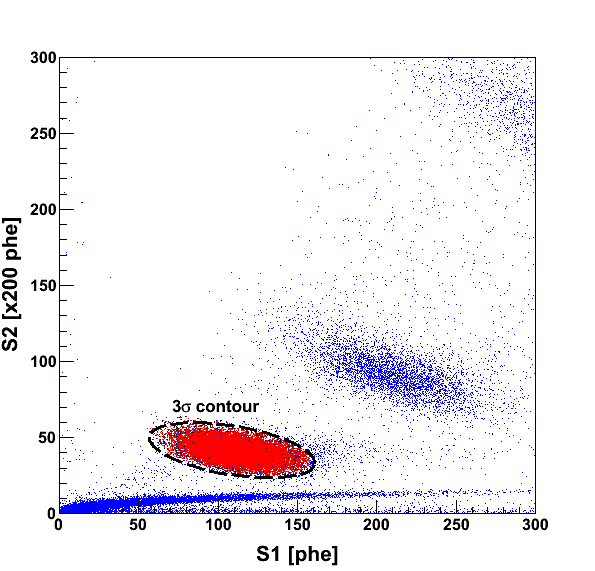
\includegraphics[height=0.375\linewidth]{plots/CES/S2vsS1_40keV.png}
%\label{fig40keV_1}}
%\subfigure[]{
%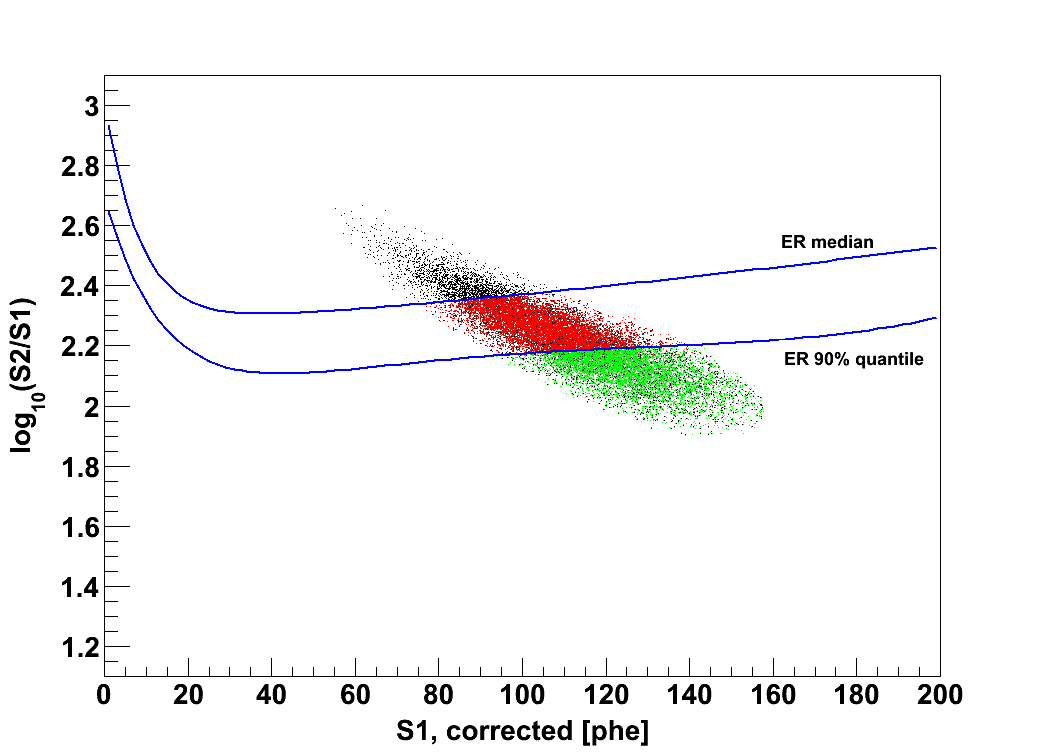
\includegraphics[height=0.375\linewidth]{plots/CES/logS2S1_40keV.png}
%\label{fig40keV_2}}
%\caption{Anticorrelation between S1 and S2 (a) and log$_{10}$(S2/S1) (b) for 40~keV line.}
%\label{fig40keV}
%\end{figure}


%\begin{figure}[!h]
%\centering
%\includegraphics[width=0.475\linewidth]{plots/AmBeCalibrationAmBe_run0708_dataMC_0-250keV.png}
%\caption{Simulated and measured energy spectra for the calibration with inelastic neutron scatters from $^{241}$Am-Be source}
%\label{figAmBeSpectra}
%\end{figure}




